\chapter{Potential sources of high-energy gamma-rays}
\label{CHAP::SOURCES}

To date, EGRET sources have been unambiguously identified with only
two major source types: blazars and pulsars (neglecting the LMC, Cen
A, the solar flare and \Gray bursts). Numerous population studies have
noted that there are coincidences between the population of
unidentified sources and catalogs of other types of sources which
exceed what should be expected from chance probability; however these
studies do not provide compelling associations for any individual 3EG
sources. Some suggested source classes are massive stars, OB
associations, supernova remnants (SNR), x-ray binaries and
micro-quasars. In addition, it seems likely that there are three
independent populations of unidentified source: those associated with
the Galactic plane, extra-galactic sources and a population of local
sources in the Gould Belt.

\section{Blazars}
\label{SEC::SOURCES::BLAZARS}

One of the most unexpected results from the EGRET mission was the
discovery of \Grays from a large number of extra-galactic
sources. Before EGRET, only one extra-galactic source had been
detected in {\Grayc}s, 3C273, based upon observations with the COS-B
satellite \citep{REF::SWANENBURG::NATURE1978}. In total, 67
high-confidence associations of EGRET sources were made with blazars,
a type of radio loud active galactic nucleus (AGN). AGN are galaxies
with a bright central core which typically outshines the $\sim10^{11}$
stars present in the Galaxy by up to three orders of magnitude. AGN
are thought to be powered by accretion of material onto a
super-massive black hole, (mass $\sim10^6M_\odot$ to
$\sim10^{9}M_\odot$). The accreting material forms a disk around the
core, at temperatures which can produce continuum emission at UV to
soft x-ray energies. AGN can form jets of relativistic charged
particles, aligned perpendicular to the plane of the accretion
disk. The mechanism responsible for forming the jet is not completely
understood. The accretion disk is surrounded by clouds of hot gas
which produce broad line emission. Far out from the core, narrow line
emission is produced in clouds of particles, possibly energized by the
jet.

AGN have been sub-classified based upon their observational
properties, with some classes being more powerful, and therefore
better studied, in different energy ranges. At \Gray energies, the
blazar subclass of AGN are powerful emitters. Blazars are
characterized by strong emission in radio (they are referred to as
radio-loud AGN), continuum emission across the spectrum, very rapid
variability on the order of hours to days and weeks, high polarization
and the ejection of ``blobs'' of material at apparent super-luminal
velocities, usually visible in radio. The blazar sub-class consists of
``BL Lac'' type objects, and flat-spectrum radio quasars
(FSRQs). These objects are distinguished on the basis of prominent
(FSQR) or weak (BL Lac) absorption/emission lines in their spectra. In
general, the lack of lines in the spectra of BL Lac objects makes it
difficult to determine their redshift, and hence distance. It also
means that they are usually identified as AGN at radio or x-ray
energies, since they are essentially featureless at optical
wavelengths. It has been suggested that all AGN can be unified by a
single model
\citep{REF::URRY::PASP1995}, and that the different observational
properties of the AGN classes arise primarily from differences in the
viewing angle with respect to the jet and the total power of the
accreting object. For example, the presence or absence of broad lines
in the spectrum depends on whether the broad line emission region is
obscured from sight by other parts of the AGN structure. Blazars are
thought to be AGN with jets aligned close to our line-of-sight. The
physics behind \Gray emission in the jet is not well known, and many
models exist. The most widely discussed models are leptonic,
synchrotron/inverse Compton models, in which synchrotron emission from
electrons in the jet produces the low energy emission (radio, optical
and soft x-ray) while inverse Compton up-scattering of the soft
synchrotron photons by the same population of electrons accounts for
the high energy emission. This model, referred to as the
synchrotron-self-Compton (SSC) model, predicts that the peak in the
power output of the IC component is correlated with the peak in the
synchrotron emission, and has been relatively successful in fitting
the emission seen from blazars. A review of leptonic emission models
can be found in \citet{REF::BOETTCHER::1999SNOWBIRD}.

The identification of some EGRET sources with blazar objects is
presented in detail in \citet{REF::VONMONTIGNY::APJ1995},
\citet{REF::MUKHERJEE::APJ1997}, \citet{REF::HARTMAN::APJS1999} and
references therein. A recent summary of the EGRET blazars can be
found in \citet{REF::MUKHERJEE::HEGRA2001}. In general,
identifications were made on the basis of positional coincidence with
known radio sources.  The blazars listed in the 3EG catalog consist
of 50 FSRQs and 17 BL~Lacs, with redshift between $z=0.03$ and
$z=2.28$. For most of these objects the \Gray emission dominates the
total luminosity at all other wavelengths. Their spectra are well fit
by a power-law with average spectral index of
$\langle\Gamma\rangle=2.2$ and no cut-off has been seen up to
10\,GeV. The average variability index of the blazars, from
\citet{REF::NOLAN::APJ2003}, is $\langle\delta\rangle=0.70\pm0.08$
with $\mathrm{RMS}(\delta)=0.27\pm0.05$, showing that they are
consistent with being variable ($\delta\rightarrow0$ for persistent
sources, and $\delta\rightarrow1$ for variable sources).

The GeV and 10\,GeV catalogs also contain a number of additional
blazar identifications. The 10\,GeV catalog suggests that there may be
a blazar identification for 3EG~J0433$+$2908 and for GeV~J0508$+$0540.  In
the time since the 3EG-catalog was published a number of
investigations have been made into individual unidentified EGRET
sources, leading to possible (or likely) blazar identifications for
them. For example, \citet{REF::MUKHERJEE::APJ2000} suggest that
3EG~J2016$+$3657 is associated with a blazar, an especially interesting
result as the source is located at low Galactic latitude
($b=0.5^\circ$), possibly making it the first blazar identified in the
direction of the plane.
% Could mention Wallace 2002 see wallace-agn-J2006-2321-01.pdf

Of the 3EG blazars, two are confirmed sources of VHE {\Grayc}s:
Markarian~421 (usually abbreviated to Mrk~421) and PKS2155$-$304. A
third confirmed VHE source, Mrk~501 is significant only in the EGRET
GeV catalog. On the other hand, there are three confirmed VHE blazars
not seen by EGRET: H1426$+$428, 1ES1959$+$650 and 1ES2344$+$514, all
BL Lac type objects. To date, no FSRQs have been detected by VHE
instruments. EGRET largely detected low-frequency peaked BL~Lacs (LBL)
and FSRQs. These objects have the peak in their synchrotron power
emission in the optical, UV or soft x-ray bands. All confirmed BL~Lac
detections in the VHE band are high-frequency peaked BL~Lacs (HBL),
with peak synchrotron power in the hard x-ray band. Correspondingly,
the peak in the inverse Compton emission is at higher energies in
HBLs, lying in the 300\,GeV to 30\,TeV range. The energy range in
which EGRET was most sensitive fell in that region of the spectrum in
which HBLs are least powerful; between the peaks of the synchrotron
and inverse-Compton emission. Therefore, EGRET was not sensitive
enough to detect many of the TeV selected BL~Lacs. The most distant
blazar detected in the VHE regime is H1426$+$428, at a redshift of
$z=0.129$. Many models predict that interactions of VHE \Grays with
the extra-galactic background light will attenuate the \Gray signal to
such an extent that sources located at distances much larger than
H1426$+$428 are not be visible in \Grays at GeV-TeV energies, with
current detector sensitivities.

In summary, it seems likely that blazars make up a considerable
fraction of the unidentified EGRET sources. Blazars are expected to be
uniformly distributed across the sky, to have flat spectra which
steepen with distance, and are characterized by extreme variability
across the spectrum from radio to TeV energies. Since the known \Gray
blazars have been readily identified with their radio, optical and
x-ray counterparts, new identifications would suggest some unusual
spectral distributions and/or obscuration, e.g.\ by the Galactic plane.

\subsubsection*{\boldmath Intergalactic \Gray absorption}

The spectra of \Grays detected from all extra-galactic sources are
altered from the intrinsic source emission spectrum by absorption of
the signal in the ambient field of intergalactic
photons. \citet{REF::NIKISHOV::JETP1961} was the first to suggest that
high-energy photons would interact with infra-red photons in
intergalactic space by photon-photon pair production. At that time,
little was known about the strength of the inter-galactic infra-red
radiation field (IIRF) and the value assumed in the calculation was
too large by three orders of magnitude. Shortly after the discovery of
the cosmic microwave background (CMB), it was realized by
\citet{REF::GOULD_SCHREDER::PRL1966} and \citet{REF::JELLEY::PRL1966}
that the universe is effectively opaque to \Grays with energy greater
than $\sim$100\,TeV. \citet{REF::GOULD_SCHREDER::PR1967} extended these
calculations to account for absorption with radio, microwave, IR and
optical photons.

The unexpected discovery of the optically violent variable quasar,
3C279, by EGRET prompted \citet{REF::STECKER::APJ1992} to suggest that
any subsequent discovery of TeV emission from the object could be used
to determine (or at least provide limits on) the density of the
IIRF. The discovery of the blazar Mrk~421 at TeV energies
\citep{REF::PUNCH::NATURE1992}, and the subsequent discovery of other
TeV blazars, has produced considerable interest in this subject
\citep[see for example][and references
therein]{REF::VASSILIEV::AP2000}.

\enlargethispage{13pt}
The threshold for a a soft photon with energy $\epsilon$ (as measured
locally) to interact with a \Gray with energy $E$ (measured locally)
at redshift of $z$ is \[\epsilon>\frac{2(m_ec^2)^2}{E(1+z)^2}
\approx\frac{0.52}{E/\mathrm{TeV}}\,\mathrm{eV.}\] for small
redshifts. For a 1\,TeV photon, this corresponds to an IR photon near
to the K-band (2\,$\mu$m). For energies above 100\,TeV the threshold
is in the CMB region. The amount of absorption a signal from a distant
source undergoes can be calculated from the pair-production
cross-section, due to Heitler, given some assumptions for the spectrum
of soft-photons \citep[see for
example][]{REF::STECKER::SSR1996}. \citet{REF::STECKER_DEJAGER::AA1998}
calculated the optical path length (or \textit{opacity}, $\tau(E,z)$)
for TeV photons from relatively small redshifts ($z\leq0.3$), which
they presented in parameterized form, valid for 1\,TeV$<E<$50\,TeV and
$z<0.3$. Figure~\ref{FIG::SOURCES::EBL} shows the opacity, from the
parameterized form, as a function of \Gray energy for three
redshifts. The change in the intrinsic source spectrum for these cases
is also shown. In each case a strong cut-off\,\footnote{Defined as the
energy at which $\tau(E,z)=1$ and the spectrum falls to 1/e of its
intrinsic value.} in the measured \Gray spectrum is predicted,
independent of the source emission spectrum. For sources at
$z\sim0.03$, like Mrk~421, the cut-off occurs at $\sim10$\,TeV,
decreasing to $\sim1$\,TeV for a more distant source, such as
H1426$+$428 at $z=0.129$.

\begin{figure}[t]
\hspace*{\fill}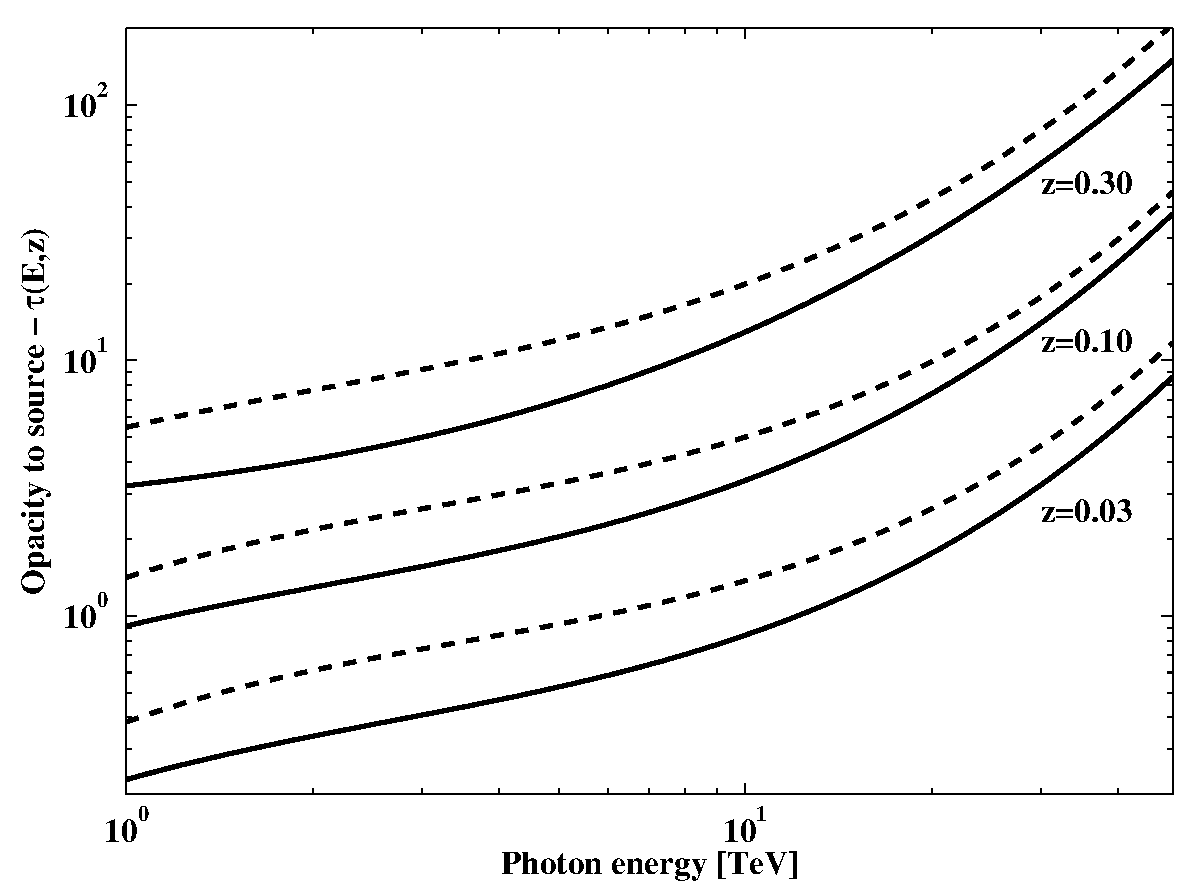
\includegraphics[angle=270,width=0.49\textwidth]{plots/chap-sources/ebl_opacity.pdf}\hspace*{\fill}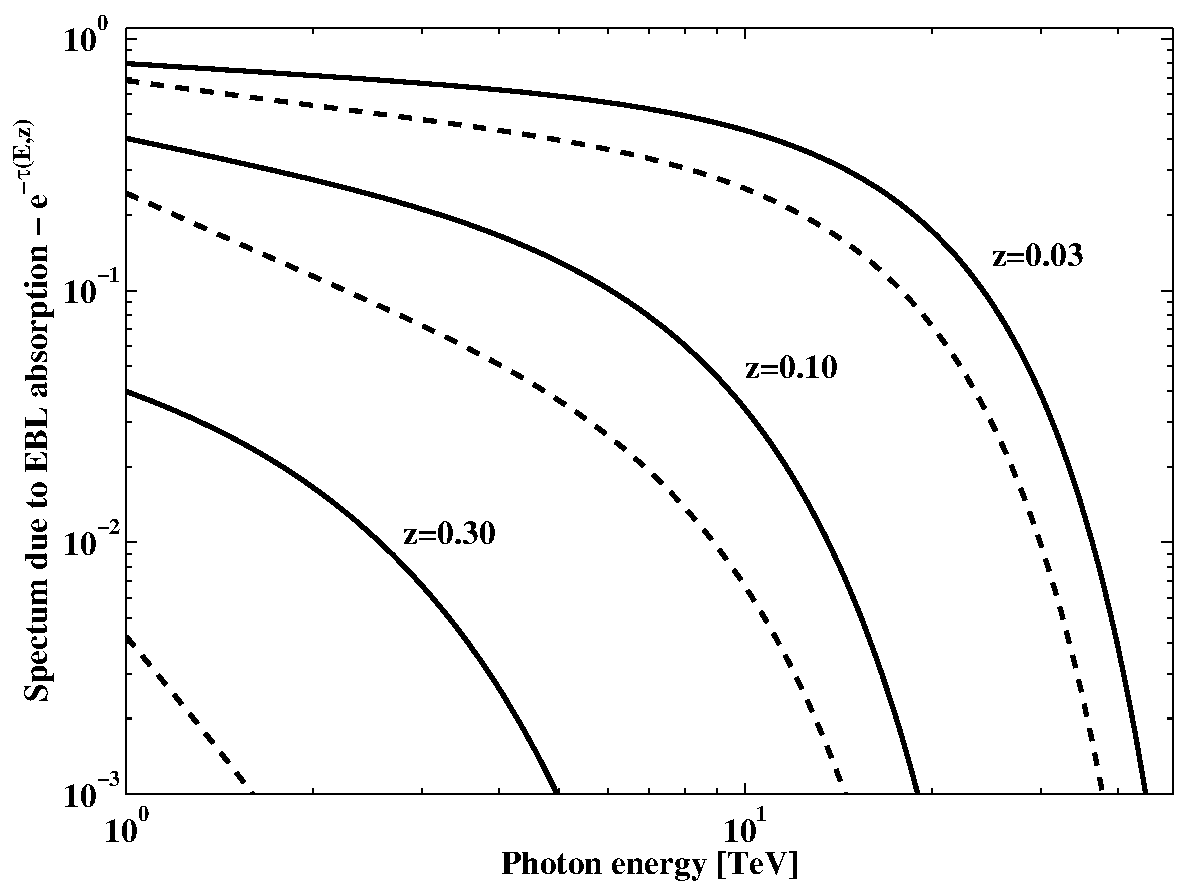
\includegraphics[angle=270,width=0.49\textwidth]{plots/chap-sources/ebl_spectrum.pdf}\hspace*{\fill}
\caption{\label{FIG::SOURCES::EBL} (Left) Optical path length, $\tau(E,z)$,
for HE \Grays from extra-galactic sources at $z=0.03$, $z=0.10$ and
$z=0.30$ from \citet{REF::STECKER_DEJAGER::AA1998}. (Right) Cut-off in
\Gray spectrum due to absorption, $\exp\{-\tau(E,z)\}$. In each case,
two curves are shown, corresponding to the two the IIRF models used by
\citet{REF::STECKER_DEJAGER::AA1998}.}
\end{figure}

Predicting VHE emission from the EGRET blazars requires the
opacity be known in the energy range $\sim$1\,GeV$<E<\sim$1\,TeV, and
for larger redshifts. For this energy range, the extra-galactic soft
photon spectrum must be estimated at optical wavelengths, where the
major contribution comes from
starlight. \citet{REF::SALAMON_STECKER::APJ1998} presented a
calculation of this function, and its implication for a number of
EGRET blazars. They did not present a parameterized form of the
function, which could be plotted here. Qualitatively, the results are
similar to the TeV case: the opacity increases with energy and
redshift. For a source at $z=1$ the opacity increases from $<10^{-2}$
at 20\,GeV to $\geq8$ at 500\,GeV. For the EGRET source 3C279
($z=0.54$) a spectral cut-off is predicted at $\sim$90\,GeV; for B1633$+$382
($z=1.81$) it is at $\sim$25\,GeV.

\section{Pulsars}
\label{SEC::SOURCES::PULSARS}

\enlargethispage{8pt}
The second largest category of identified MeV \Gray point sources is
pulsars. The 3EG catalog lists five associations between pulsars and
EGRET point sources: Crab, Vela, Geminga, PSR~B1706$-$44 and
PSR~B1055$-$52 \citep{REF::NOLAN::AAS1996}.
\citet{REF::KASPI::APJ2000} report evidence of pulsations from
PSR~B1046$-$58 (3EG~J1048$-$5840) at the $3.1\sigma$ level. PSR~B1951$+$32,
was identified as a pulsar in EGRET data
\citep{REF::RAMANAMURTHY::APJ1996}, although it does not appear in the
3EG catalog\footnote{The pulsar is depicted at the correct location in
the map of sources, figure~4, in
\citet{REF::HARTMAN::APJS1999} while it is missing from
figure~\ref{FIG::INTRODUCTION::3RDEGRET} in
chapter~\ref{CHAP::INTRODUCTION}, which was generated directly from
the electronic version of the 3EG catalog.} (it fell below the
$5\sigma$ requirement for detection on the Galactic
plane). \citet{REF::RAMANAMURTHY::APJ1995} present results of
pulsations from PSR~B0656$+$14 at the $3.6\sigma$ level, although
again it is not a 3EG source. In an interesting analysis of a source
that contains two possible candidates, \citet{REF::KUIPER::AA2000}
show evidence for pulsations from PSR~J0218$+$4232 at the 3-4$\sigma$
level which is coincident with 3EG~J0222$+$4253, with sufficient \Gray
excess remaining to also accommodate the detection of the blazar 3C66A
in that field. \citet{REF::HALPERN::APJ2001::2227PAPER2} report
observations of the region near 3EG~J2227$+$6122 in x-ray, optical and
radio and suggest an association with an x-ray/radio pulsar
PSR~J2229$+$6114. Lacking an appropriate ephemeris covering the EGRET
observations, they were not able to perform a pulsed search at MeV
energies -- but, since no other x-ray counterpart is found to be
consistent, they claim it is more conservative to accept the
association than to reject it. Finally, PSR~B1509$-$58 is also a \Gray
pulsar; pulsations have been detected at lower energies by the OSSE
and BATSE experiments on CGRO but not by EGRET
\citep{REF::ULMER::APJS1994}.

The unambiguous associations, listed above, were made by searching for
significant pulsations in the \Gray data, given a contemporaneous
pulsar ephemeris (phase, frequency and frequency derivatives), usually
determined from radio observations\footnote{Or from ROSAT x-ray
observations in the case of the radio-quiet Geminga
pulsar.}. Additionally, blind searches for pulsations were performed
for those sources with sufficient detected counts. The median number
of counts detected from unidentified sources on the plane is
$\sim400$, insufficient for a blind search considering that the
PSR~B1046$-$58, $3.1\sigma$ identification was made with $\sim350$
counts and a \textit{known} pulsar ephemeris.

Since mid-1997, the sensitive Parkes Multibeam Survey
\citep{REF::MANCHESTER::MNRAS2001} has detected a large number of new
radio pulsars at $|b|<6^\circ$. Some of these have been shown to
be coincident with unidentified EGRET sources
\citep{REF::MANCHESTER::NSSR2002}. Due to pulsar glitches, the
ephemerides for these objects cannot, in general, be extrapolated
back to the period of the EGRET observations and definitive
associations cannot be made. Other pulsar associations for
unidentified 3EG sources have also been suggested
\citep{REF::ROBERTS::APJ2002, REF::BRAJE:APJ2002,
REF::ROBERTS::APJ2001, REF::DAMICO::APJ2001}.  A recent paper by
\citet{REF::TORRES::PR2003} reviews the current status of pulsars
coincident with EGRET sources.

The six identified pulsars listed as sources in the 3EG catalog are
all located close to the Galactic plane, at $|b|<6^\circ$. They have
hard spectra, with mean $\langle\Gamma\rangle=1.89$; only the Crab has
a $\Gamma>2.0$. The sources are persistent over all viewing periods,
and are consistent with having a constant flux, within the 10\%
systematic errors due to possible errors in the calibration of the
instrument over the long duration of the mission. The mean variability
index from \citet{REF::NOLAN::APJ2003} is
$\langle\delta\rangle=0.11\pm0.02$ with $\mathrm{RMS}(\delta)<0.07$.

The power to produce emission from pulsars comes from the slowing of a
spinning neutron star. \citet{REF::GOLDREICH_JULIAN::APJ1969} showed
that if a spinning neutron star were to exist in a vacuum, a huge
surface electric field would exist parallel to the magnetic field
lines ejecting charged particles from the neutron star surface quickly
forming a co-rotating plasma, called the magnetosphere, distributed to
balance the electric and magnetic fields. Such a co-rotating plasma is
not completely possible, however, since portions of the plasma, beyond
what is known as the light-cylinder, would be forced to move faster
than the speed of light. The field lines become open at this point and
particles can be ejected from the magnetosphere. Under certain
circumstances, charges cannot be easily replenished from the surface
of the neutron star and the out-flow of particles from the system can
lead to a deficit in the charge density in certain regions of the
magnetosphere; just above the surface of the neutron star at the pole
(the ``polar cap'') and along the edge of the closed magnetosphere
near to the light cylinder (the ``outer gap''). In these regions, the
electric field is not constrained by the plasma to be perpendicular to
the magnetic field and particle acceleration can occur.

Two main models for high-energy \Gray emission from pulsars have been
proposed. Each predicts a different ratio for the populations of
radio-loud to radio-quiet pulsars and different levels of emission in
the VHE \Gray regime. The models differ on where the acceleration
takes place, in the \textit{polar cap} or the \textit{outer gap}.
\citet{REF::HARDING::HEGRA2001} presents an overview of each model and
gives references to detailed descriptions. These models fit the hard
spectra for those pulsars detected by EGRET from radio through MeV
energies, both for young pulsars (such as the Crab) and older pulsars
with weaker magnetic fields (such as Vela). They can also account for
radio-quiet pulsars such as Geminga.

In the \textit{polar cap} model, the gap forms when the electric field
is insufficient to overcome the potential that binds ions to the
stellar surface -- a low surface temperature also contibutes
\citep{REF::RUDERMAN_SUTHERLAND::APJ1975}. If the angular momentum and
magnetic field are opposite at the pole, the magnetosphere in the
region of the pole contains a positively charged plasma which cannot
be replenished with ions from the surface, resulting in a
gap. Accelerated particles interact through inverse Compton scattering
with thermal x-rays from the surface of the neutron star and curvature
radiation (CR) emitted as the charged particles follow the curved
field lines. These IC up-scattered photons and CR give rise to
particle/photon cascades through pair-production. As the cascade is
accelerated further, the density of charged particles increases to the
point that the electric field is screened, closing the gap. At this
point, no further acceleration is possible. The huge magnetic field in
the accelerating region allows single photon pair-production
($\gamma\rightarrow e^\pm$) and photon splitting ($\gamma\rightarrow
2\gamma$) that gives rise to a sharp, super-exponential, cut-off in
the spectrum of \Grays produced. The cut-off occurs at several GeV for
most young pulsars and as high as 50\,GeV for older pulsars with
weaker field strengths. The \Gray emission forms a beam that is
largely coincident with the radio beam; this model does not predict
the occurrence of large numbers of radio-quiet pulsars (such as
Geminga). Accounting for the size of the beam and making assumptions
about the population of pulsars in the Galaxy, the polar cap model
predicts 19 radio-loud and 4 radio-quiet pulsars detectable by EGRET
\citep{REF::HARDING::SSRNS2003}.

In the \textit{outer gap} model, acceleration occurs in a charge
depleted region much further from the surface of the neutron star,
which cannot be replenished from the stellar surface. Pair-production
in the gap must provide the current needed for acceleration. In young
pulsars the pairs are produced by interaction of CR from the
accelerated particles and non-thermal synchrotron x-rays from the same
pairs. In older pulsars, up-scattering of the flux of thermal x-rays
from the hot surface of the neutron star is responsible for pair
production. As in the polar cap model, at some point the electric
field is screened by the pairs and acceleration stops. Since the
magnetic field is orders of magnitude lower than the polar-cap region,
single photon interactions are negligible and a slower cut-off in the
primary \Gray spectrum is predicted due to the upper limit in the
accelerated particle spectrum. An additional, VHE ($>$100\,GeV)
component is predicted from IC up-scattering of infra-red photons,
even from pulsars with the highest magnetic fields. Recent
predictions give a flux at VHE energies below the sensitivity of
current ground-based detectors. The beam of MeV
\Grays is not coincident with the radio beam (which comes from the
polar region) but is considerably larger in solid angle. In this
model, it is possible for the observer's line-of-sight to intersect
either or both (or neither, but that would be uninteresting) of these
beams giving a larger population of radio-quiet \Gray pulsars.
\citet{REF::ZHANGZHANGCHENG::AA2000} predict that, 10 radio-loud and
22 radio-quiet pulsars should be detectable by EGRET.

In summary, 6$-$10 pulsars have been associated with EGRET
sources. Their source characteristics are steady (but pulsed) fluxes,
flat spectra that steepen above 10\,GeV and Galactic distributions.
Pulsar models suggest that radio-quiet pulsars could account for a
large fraction of the unidentified sources. VHE emission is expected
from the outer gap model, but, given the parameters of the EGRET
pulsars, the predicted flux is too low to detect at the
sensitivity of current VHE observatories. However, this small sample
of 100\,MeV pulsars may not be typical and given the large
uncertainties in pulsar mechanisms, VHE emission is probable at some
level.

\section{Supernova Remnants} 
\label{SEC::SOURCES::SNR}

The 3EG catalog lists a number of possible positional associations
with known supernova remnants (SNR), such as IC443, W28, W44,
$\gamma$~Cygni, CTA1 and G347.3$-$0.5
\citep{REF::ESPOSITO::APJ1996}. Additionally, a number of suggestions
for SNR associations with unidentified sources have since been made
\citep{REF::COMBI::AA2001, REF::ROBERTS::APJS2001}. 
\citet{REF::ROMERO::AA1999} present a list of 27 SNR coincident 
with 22 EGRET sources (some sources have more than one possible SNR
candidate). However, there are no unambiguous identifications of SNR
with any individual EGRET sources. \citet{REF::TORRES::PR2003} present
a recent review of supernova coincident with EGRET sources.

It has long been suspected that SNR could be the acceleration sites of
cosmic rays \citep{REF::GINZBURG::BOOK1964}. The mechanism for
producing these high energy particles is diffusive shock acceleration
(DSA) of charged particles in the blastwave of the expanding remnant,
which can allow acceleration of particles to energies of
$10^{14}-10^{15}$\,eV per nucleon. The flux of cosmic rays observed at
the Earth is isotropic; the Galactic magnetic field ensures that no
hint of the origin can be inferred from the direction of the particles
themselves, except possibly for those of the highest
energy. Production of high-energy \Grays which is expected to
accompany the acceleration could finally identify the sites and
mechanisms responsible.

A typical supernova ejects a shell of mass $\sim1M_\odot$ into the
interstellar medium (ISM) at speeds of $\sim10^4$\,km\,s$^{-1}$,
giving a kinetic energy budget of $\sim10^{51}$\,erg to the
ejecta. The shell moves through the ISM at speeds much greater than
the local speed of sound (10-100\,km\,s$^{-1}$), creating a strong
shockwave, which sweeps the interstellar material with it. After a
relatively short period (typically few hundred years) of uniform
expansion, the mass of material swept up becomes comparable to that of
the original ejected shell. The blastwave then enters the so-called
Sedov-phase, in which radiative losses are small in comparison to the
internal energy of the shock, and starts to slow and cool over
timescales of $\sim10^4$\,yr. When the shock reaches speeds of
$\sim200$\,km\,s$^{-1}$, radiative processes quickly cool the shell
which eventually falls to the density of the ISM and loses its
identity \citep{REF::WOLTJER::ARAA1972}. It is during the Sedov phase
that conditions in the shock are correct for particle acceleration to
occur. The Green Catalog of SNR \citep{REF::GREEN::WEB2001} contains a
total of $\sim230$ identified SNR, detected through radio and x-ray
observations. They generally lie along the plane, but some, such as
SN~1006, lie at latitudes up to $b=15^\circ$.

The theory of diffuse shock acceleration seems to have been
independently arrived at by \citet{REF::KRYMSKII::DOSSR1977},
\citet{REF::AXFORD::ICRC1977}, \citet{REF::BELL::MNRAS1978} and 
\citet{REF::BLANDFORD_OSTRIKER::APJ1978}, although the idea was
around in less developed forms for some time before that
\citep{REF::FERMI::PR1949}. \citet{REF::DRURY::RPP1983} presents a
review of the process.  Charged particles in the plasma on both sides
of the shock front are constrained to move along the magnetic field
lines and can scatter isotropically from irregularities in the
magnetic field. If they are injected into the region of the shock with
sufficient velocity such that there is negligible interaction with the
shock front, they can be repeatedly scattered across the shock front
between the up-stream and down-stream regions. Since an isotropic
distribution in one region appears to be relativistically beamed to an
observer co-moving with the plasma in the other region, the particle
gains energy when it is scattered isotropically in the second region
after crossing the shock. The particle gains energy exponentially on
each crossing. There is a small probability on each crossing into the
downstream region that the particle will not re-cross, since the shock
front is advancing through space. The probability of a particle
crossing the shock more than $n$ times falls exponentially with
$n$. These two exponential relations give rise to the power-law energy
distribution that is characteristic of shock acceleration. DSA models
have evolved to accommodate spherical shock fronts, various injection
models, magnetic field configurations and to account for the reaction
of the accelerated particles on the development of the shock.

Accelerated protons are expected to produce a \Gray signal through
intermediate pion production and decay
$p+p\rightarrow\pi^0\rightarrow2\gamma$ \citep{REF::DAV::AA1994}.
Emission from $\pi^0$ decay is expected to peak soon after the
beginning of the Sedov phase and stays largely constant until the
radiative phase dissipates the energy of the shock material. It is
expected that in regions where the SNR shock interacts with a medium
of higher density than the ISM, such as large, dense molecular clouds,
the $\pi^0$ flux will be enhanced. The spectrum of
\Grays extends from 100\,MeV to 10\,TeV. \citet{REF::DAV::AA1994}
predict that \Gray emission should be clearly detectable by
ground-based instruments at TeV energies. There have been two
suggestions, that $\pi^0$ decay has been seen at TeV energies.
\citet{REF::ENOMOTO::NATURE2002} suggest that the broadband
spectrum of emission from the SNR RX~J1713.7$-$3946, including
observations at TeV energies by the CANGAROO instrument, is best
fitted by a pion spectrum, although the result is controversial
\citep{REF::REIMER_POHL::AA2002, REF::BUTT::NATURE2002}. 
\citet{REF::AHARONIAN::AA2001}
present evidence of a $\pi^0$ spectrum from observations of
the SNR Cassiopeia~A, although the spectrum is consistent with
an electron induced spectrum at a 15\% level.

In addition to \Gray production through proton interactions, electrons
accelerated in the shock are responsible for non-thermal emission,
through bremsstrahlung, inverse-Compton up-scattering of the cosmic
microwave background, local infra-red/optical photons or radiation
from the SNR itself and through synchrotron emission in the magnetic
field of the SNR. These processes are generally considered to be
responsible for the radio and x-ray emission from shell type supernova
remnants.  As mentioned above, it can also explain \Gray emission in
the MeV and TeV ranges for some SNR. It is widely believed that the
bulk of cosmic radiation below $10^{14}$\,eV originates in supernova
remnants in the Galaxy. It would be unexpected if such sources were
not apparent as major components of the VHE \Gray sky. There are major
uncertainties in these sources (apart from the total energetics) so
that the unidentified EGRET sources may be important pointers to the
exact locations of the acceleration sites.

\section{Pulsar Wind Nebulae}
\label{SEC::SOURCES::PWN}

Of the $>200$ SNR in \citet{REF::GREEN::WEB2001}, approximately ten
belong to an anomalous class of remnant called Pulsar Wind Nebulae
(PWN), and often referred to as \textit{plerions} or
\textit{Crab-like} SNR \citep[see][]{REF::CHEVALIER::APJ2000}. 
While typical SNR are characterized by a shell-type structure with a
steep spectrum of non-thermal radio emission and a shell of x-ray
emission, PWN emission is dominated by a central core nebula, with
strong non-thermal optical and x-ray emission and a harder radio
spectrum. The x-ray and radio emission from the core region is the
result of synchrotron radiation from very energetic electrons in the
strong magnetic fields that thread the nebula. The short synchrotron
cooling time of these electrons requires that the nebula be resupplied
by the energetic particles being ejected from the pulsar. The PWN
morphology is complex, with glowing filamentary structures where
synchrotron emission is enhanced and cooler outer regions which show
evidence of emission lines. \Gray emission from the synchrotron nebula
can occur through inverse-Compton up-scattering of the synchrotron
photons (up to TeV energies) by high-energy electrons. \Gray emission
in the MeV range can also result for shock-acceleration of the
electron population to higher energies. \citet{REF::ROBERTS::NSSR2002}
discuss PWN candidates at MeV energies and possible emission
mechanisms.  It is unlikely that PWN account for a large number of the
unidentified 3EG sources, since so few have been found in the Galaxy;
the discovery of a new PWN at VHE energies would be an important
first.

\section{Other source associations at low Galactic latitudes}
\label{SEC::SOURCES::GALACTIC}

\citet{REF::GRENIER::TEXAS2002} and \citet{REF::ROMERO::AA1999}
discuss other possible Galactic sources for unidentified EGRET
sources. Some of the possibilities are summarized briefly below.

\subsection{Massive Stars}
\label{SEC::SOURCES::MASSIVESTARS}

Particle acceleration through diffusive shock acceleration occurs at
the terminal shocks around all stars, including the Sun. Massive stars
are expected to accelerate particles to energies at which they could
up-scatter the UV radiation from the star to \Gray energies. None of
the many O-type\footnote{Stars are classified by their spectral
characteristics into classes that reflect their surface
temperatures. From hottest (blue) to coolest (red) the sequence goes
O-B-A-F-G-K-M.} stars in our neighborhood have been observed by
EGRET. Binary systems with a massive stars would provide stronger
shocks and a larger target of UV radiation. Wolf-Rayet (WR) star
systems, with a massive O-type star and companion, where the companion
has stripped the star's outer layers are also possibilities. The WR+O
system Cyg~OB2~No.5 has been suggested as a candidate for
3EG~J2022$+$4317 \citep{REF::BENAGLIA::AA2001}, a source observed in
this TeV survey. \citet{REF::ROMERO::AA1999} present eleven WR stars
which have positional coincidence with six 3EG sources and six Of-type
stars coincident with four 3EG sources. As yet, there are no detailed
models of VHE emission from massive stars.

\subsection{OB Associations}
\label{SEC::SOURCES::OB}

OB associations are collections of massive O- and B-type stars which
are the sites of star formation. OB associations have a larger density
of pulsars and SNR than the rest of the Galaxy\footnote{In an instance
of humorous astrophysical nomenclature, SNR embedded in OB
associations are often referred to as SNOBs.}. The strong interstellar
winds from the massive O-type stars, possible SNR shock fronts, pulsar
winds and massive molecular clouds make OB associations good
candidates for \Gray production \citep{REF::KAARET::APJ1996}. 
\citet{REF::ROMERO::AA1999} detail 22 unidentified 3EG sources that have 
positional coincidences with known OB associations.

\subsection{Gould Belt}
\label{SEC::SOURCES::GOULD}

\enlargethispage{12pt}
The Gould Belt is a local collection of star forming regions (OB
associations). The origin of the Gould Belt is not completely
understood. It is known that it is a relatively young structure at
30\,Myr, which our solar system (age 5\,Gyr) happens to be ``passing
through'' -- the speed of the solar system in the Galaxy is larger
than the average Gould Belt speed, so eventually we will pass beyond
the Belt. The Belt was first identified in the mid 1800s, when it was
noticed that the bright stars tend to trace a plane inclined to
20$^\circ$ to the Galactic plane. The plane is roughly elliptical in
shape with dimensions of 1000\,pc $\times$ 600\,pc. The solar system
is $\sim150$\,pc from the center
\citep{REF::LEDREW::ASTRONOTES99}. The Belt was mapped by
\citet{REF::STOTHERS::AJ1974}, who noted that the density of massive
O-type to B2-type stars, within 400\,pc, is three times larger in the
Belt than in the Galactic plane. 

Diffuse \Gray emission associated with the Gould Belt was first
recognised in data from the SAS-2 experiment, in the region of the
Galactic anti-center where the Belt lies furthest from the plane
\citep{REF::THOMPSON::APJ1977}. More recently, it has been shown that
the distributions of all steady, unidentified 3EG sources are best
fitted by a combination of three population classes. In addition to
the Galactic plane and extra-galactic populations,
\citet{REF::GEHRELS::NATURE2000} suggest there is a population
correlated with the Gould Belt, 47 unidentified sources are possibly
associated with this population. \citet{REF::NOLAN::APJ2003} give the
mean variability index for the 33 possible Gould Belt sources at
$|b|>5^\circ$ as $\langle\delta\rangle=0.49$, which they refer to as a
``moderately low value'', inconsistent with a purely pulsar
population. Not enough is known about these OB sources to make any
predictions of VHE emission.

\subsection{X-ray binaries and micro-quasars}
\label{SEC::SOURCES::XRAYBINARY}

%\enlargethispage{12pt}
High mass x-ray binaries, consisting of a pulsar and large companion
star, can accelerate electrons to TeV energies, resulting in x-ray
synchrotron emission and possibly \Grays up to TeV energies through
inverse-Compton up-scattering. \citet{REF::KIRK::APP1999} suggest that
TeV \Gray emission could be present in the PSR~B1259$-$63
system. \citet{REF::KAARET::APJ2000} suggest that 3EG~J0634$+$0521, a
source considered in this TeV study, is associated with the source
SAX~J0635$+$0533, a system containing a 33\,ms x-ray selected pulsar and
a large B-type star.

\citet{REF::KNIFFEN::APJ1997} suggest that the \textit{second} EGRET
catalog source 2EG~J0241$+$6119 is associated with the x-ray binary
source LSI$+$61$^\circ$\,303. This source is remarkable for its
periodic radio outbursts, on average every 26.5 days, due to the
orbital motion, with a possible modulation every 4.4\,yr
\citep{REF::GREGORY::APJ2002}. The third EGRET catalog source, 
3EG~J0241$+$6103 (also in this study) is displaced from the x-ray source
to the extent that the association is barely possible at the 95\%
confidence level.

At TeV energies, Cen~X-3 has been recently reported as a \Gray source
at the $>6\sigma$ level \citep{REF::CHADWICK::APJ1998}. A tentative
signal was reported by the HEGRA group from the micro-quasar
GRS~1915$+$105 \citep{REF::AHARONIAN::ECRS1997}. Although these claims
have not been confirmed, they give credence to the possibility that
these classes of source are emitters of VHE {\Grayc}s.

\section{Possible extra-galactic associations}
\label{SEC::SOURCES::EXTRAGALACTIC}

\citet{REF::TORRES::BOOK2003} give a review of possible extragalactic 
\Gray sources. Some possible source types are summarized below.

\subsection{Galaxy Clusters}
\label{SEC::SOURCES::CLUSTERS}

Recently, \citet{REF::KAWASAKI::APJ2002} have suggested that galaxy
clusters could be candidates for unidentified EGRET sources at high
latitude. Preliminary evidence was presented by
\citet{REF::COLAFRANCESCO::GAMMA2001} which suggests that there is a
statistical correlation between the 3EG sources at high latitude and
the clusters from the Abell catalog of clusters
\citep{REF::ABELL::APJS1989} at the $\sim3\sigma$ level. 
\citet{REF::SCHARF::APJ2002} report a correlation, also at a 
$\sim3\sigma$ level, between the EGRET sky-map of raw photons (they
considered only those with $|b|>45^\circ$) and the Abell
catalog. \citet{REF::REIMER::APJ2003} stacked (summed) the EGRET
excess photon maps for the regions around 58 of the most prominent
clusters to form one single map for the population of clusters, which
reveals no evidence for emission. They conclude that the
\citet{REF::COLAFRANCESCO::GAMMA2001} and  \citet{REF::KAWASAKI::APJ2002}
analysis were likely to explained by systematics and that their
analysis must be reconciled with the analysis by 
\citet{REF::SCHARF::APJ2002}. The potential for VHE emission from such
sources is unclear, but they would certainly be steady sources.

\subsection{Starburst Galaxies}
\label{SEC::SOURCES::STARBURST}

Starburst galaxies are characterized by a significantly enhanced rate
of star formation, and hence are rich in supernova explosions, when
compared to a normal galaxy such as the Milky Way. As a consequence
they are expected to have a high density of cosmic-rays, larger by a
factor of two orders of magnitude than the CR density of our galaxy
\citep[see][]{REF::VOLK::UVGR2003}. Consequently, significant \Gray
emission is predicted in the VHE regime. EGRET did not detect any
starburst galaxies, but set upper limits on emission on a number of
them \citep{REF::BLOM::ALC1999}. OSSE marginally detected weak
emission from NGC~253 \citep{REF::BHATTACHARYA::APJ1994}, a starburst
galaxy that has subsequently been shown to emit VHE \Grays by the
CANGAROO collaboration \citep{REF::ITOH::AA2003}. Starburst galaxies
are considered as strong candidates for VHE emission, but, because of
their proximity and prominance at other wavelengths, it is unlikely
that they could be associated with the unidentified sources.

\subsection{Radio Galaxies}
\label{SEC::SOURCES::RADIOGAL}

Centaurus~A, a radio galaxy at $z=0.0018$, appears in the 3EG catalog
as a source. Its flux is listed as
$(13.6\pm2.5)\times10^{-8}$\,cm$^{-2}$s$^{-1}$, which implies a
luminosity of $\sim10^{41}$\,erg\,s$^{-1}$, five orders of magnitude
lower than the detected blazars. Additionally, Cen~A was reported as a
VHE source at a 4.6$\sigma$ level by \citet{REF::GRINDLAY::APJ1975}.
This early report, which predates development of the imaging
technique, was made at a time of enhanced emission from Cen~A at all
wavelengths. No further VHE observations have been made during such an
active state, and it is difficult to evaluate the claim
\citep[see for example][]{REF::CARRAMINANA::AA1990}.

Although the population of known radio galaxies is $\sim1000$ times
larger than that of blazars, the smaller flux, if it is typical of
radio galaxies, explains why Cen~A is the only radio galaxy in the 3EG
catalog; further objects likely have fluxes below the sensitivity of
EGRET. Having said that, two other radio galaxies have been suggested
as associations for 3EG sources: \citet{REF::MUKHERJEE::APJ2002}
suggest that NGC~6251 as a counterpart for 3EG~1621$+$8203 and
\citet{REF::COMBI::APJ2003} report the discovery of a radio galaxy in
the error box of 3EG~J1735$-$1500.  At TeV energies, the HEGRA
collaboration have recently reported the discovery of M87 at a
$>4\sigma$ level \citep{REF::AHARONIAN::AA2003::M87}.

\section{Potential of VHE emission from unidentified 3EG sources}
\label{SEC::SOURCES::VHE3EG}

In light of these source classifications, it is possible to make some
predictions about the potential of detecting VHE emission from the
unidentified EGRET sources.

At low Galactic latitudes, it is likely that a large number of the
persistent, non-variable sources are radio-quiet pulsars. The
outer-gap model of emission, which favors a high number of radio-quiet
pulsars, suggests that VHE \Gray emission should take place, but the
parameters of the known pulsars place the level of emission below the
sensitivity of current IACTs, at least for the amount of observation
time that can be devoted to a single source in a survey (typically
5-10\,hours). To date, VHE emission has not been seen from the known
isolated pulsars. Of course, if a new class of pulsar lies undetected
in the population of Galactic EGRET sources, such as was the case with
Geminga, then a portion of model phase space could be opened up which
would allow for VHE emission.

The most likely Galactic sources of VHE {\Grayc}s, at least on the
basis of the known VHE sources, are PWN and supernovae. Three PWN have
been detected, they are expected to be persistent and
non-variable. Since a relatively small number of PWNs have been
identified in x-ray and radio observations, it seems unlikely that
they are associated with a large number of the EGRET
sources. Shell-type supernova have been identified in the fields of
many EGRET sources, and have also been detected by ground-based
instruments. The detection of RX~J1713.7$-$3946 at a significant level
took a 45\,hr.\ observation with the CANGAROO telescope,
\citep{REF::MURAISHI::AA2000}, SN1006 was detected with 28\,hrs.\ of
data \citep{REF::TANIMORI::APJ1998} and Cas~A in 232\,hrs.\ of
observations with the HEGRA IACT array
\citep{REF::AHARONIAN::AA2001}. These particular sources would not be
detectable at a significant level in a survey observation, but there
could be other stronger sources not yet identified as PWN.

Recently, the HEGRA group detected the first unidentified VHE source,
in the Cygnus region of the sky \citep{REF::AHARONIAN::AA2002::UNID}.
Again, the discovery was made on the basis of a deep observation:
113\,hrs. The source has been associated with an OB association in
Cygnus \citep{REF::BUTT::APJ2003}, although other identifications have
also been suggested \citep{REF::MUKHERJEE::APJ2003}. This association
is intriguing: OB associations have not generally been targeted for
HE or VHE emission and their complex morphology suggests that there may be
large differences between the VHE emission from one to another,
depending on the density and distribution of SNR, large stars and
stellar winds they contain. \citet{REF::ROMERO::AA1999} have listed 22
unidentified 3EG sources that have positional coincidences with known
OB associations. Potentially, some of these may be VHE \Gray emitters.

Of the variable and non-persistent Galactic sources, high mass x-ray
binaries (HMXB) and micro-quasars may be VHE \Gray sources and several
models have been proposed predicting such emission. Indeed, Cen~X-3
has been claimed as a VHE source from observations with the Durham
Mark 6 telescope \citep{REF::CHADWICK::1998}. The VHE signal was
consistent with being non-variable (but based on only 10\,hrs of
observations), in contrast to the EGRET counterpart which was seen to
vary significantly in intensity. Taken at face value, this result
indicates that HMXBs may be candidates for detection in the survey,
but the result has not yet been confirmed.  The negative results from
ground-based surveys of binary systems, such as
\citet{REF::HALL::APJ2003}, does not support the earlier optimism that
binaries might be an important class of VHE sources.

At all Galactic latitudes, blazars are expected to make up some
fraction of the unidentified sources. The EGRET blazar catalog
overlaps somewhat with the VHE BL~Lacs. No FSRQ, which make up the
majority of the EGRET blazars, has been seen in the VHE regime. Of the
EGRET BL~Lacs, it has been the weaker sources which have been those
that are visible to ground-based instruments. Given the extreme
spectral and flux variability inherent in that these sources, it is
possible that a EGRET blazar may be visible at TeV energies during a
flaring episode. Of course, catching a blazar in an extreme flaring
episode is unusual without regular monitoring of the source. The data
for this survey were not analyzed for flaring during the period of
observations, and hence follow-up observations were not made if
flaring was present. In addition, BL~Lacs at redshifts greater than
$0.129$ have not been detected at VHE energies, with the exception of
3C66A which some have regarded as spurious.

In summary, on the basis of the known source types, the motivation for
the discovery of VHE \Grays from unidentified EGRET sources is largely
exploratory. The unidentified sources have remained largely mysterious
since their discovery. The story of the first unidentified source,
Geminga, illustrates that new and unexpected source classes may be
represented in the 3EG catalog and perhaps in the VHE sky. These will
only be identified by observation in different energy regimes.  At
very least, the 3EG catalog presents a list of sources which have
emission closest in energy to the VHE regime. Unlike radio and x-ray
selected sources, they are not too numerous, and present a manageable
starting point for VHE observations.
